\documentclass[11pt,a4paper]{article}
\usepackage[margin=0.75in]{geometry}
\usepackage{hyperref}
\usepackage{pdfpages}
\usepackage{bookmark}
\usepackage{xcolor}

\hypersetup{
    colorlinks=true,
    linkcolor=blue,
    bookmarks=true,
    bookmarksopen=true,
    pdftitle={NMAMIT Complete Source Archive - All Input Files},
    pdfauthor={NMAM Institute of Technology}
}

\begin{document}

% ========== TITLE PAGE ==========
\begin{titlepage}
\centering
\vspace*{2cm}
{\Huge\bfseries COMPLETE SOURCE ARCHIVE\par}
\vspace{1cm}
{\Large\bfseries ALL Original Input Files\par}
\vspace{2cm}
{\Large NMAM Institute of Technology, Nitte\par}
\vspace{0.5cm}
{\large IV Semester B.E./B.Tech Question Papers\par}
\vspace{3cm}

{\Large\bfseries Contents of This Archive:\par}
\vspace{1cm}

\begin{itemize}
\item \textbf{Part 1:} MSE Papers Scanned Images (20 pages)
\item \textbf{Part 2:} MSE-II Source Papers (8 pages)
\item \textbf{Part 3:} Source Exam Bank (33 pages)
\item \textbf{Part 4:} Exam Question Bank with MCQs (16 pages)
\item \textbf{Part 5:} Individual Subject Papers (9 pages total)
  \begin{itemize}
  \item Linear Algebra July 2023 (2 pages)
  \item DAA July 2023 (2 pages)
  \item Microprocessor July 2023 (1 page)
  \item SEPM July 2023 (1 page)
  \item Linear Algebra June 2022 (2 pages)
  \item DAA June 2022 (1 page)
  \end{itemize}
\end{itemize}

\vspace{2cm}
{\large\textbf{Total: 86 Pages of All Source Materials}\par}
\vspace{0.5cm}
{\large\textit{Note: This PDF contains all PDFs you provided as input.\\
WhatsApp images are included in the scanned papers section.}\par}

\vfill
\end{titlepage}

% ========== PART 1: SCANNED IMAGES ==========
\bookmark[dest=part1,level=0]{PART 1: MSE Papers Scanned (20 pages)}
\hypertarget{part1}{}
\includepdf[pages=-]{mse papers.pdf}

% ========== PART 2: MSE2 SOURCE ==========
\bookmark[dest=part2,level=0]{PART 2: MSE-II Source Papers (8 pages)}
\hypertarget{part2}{}
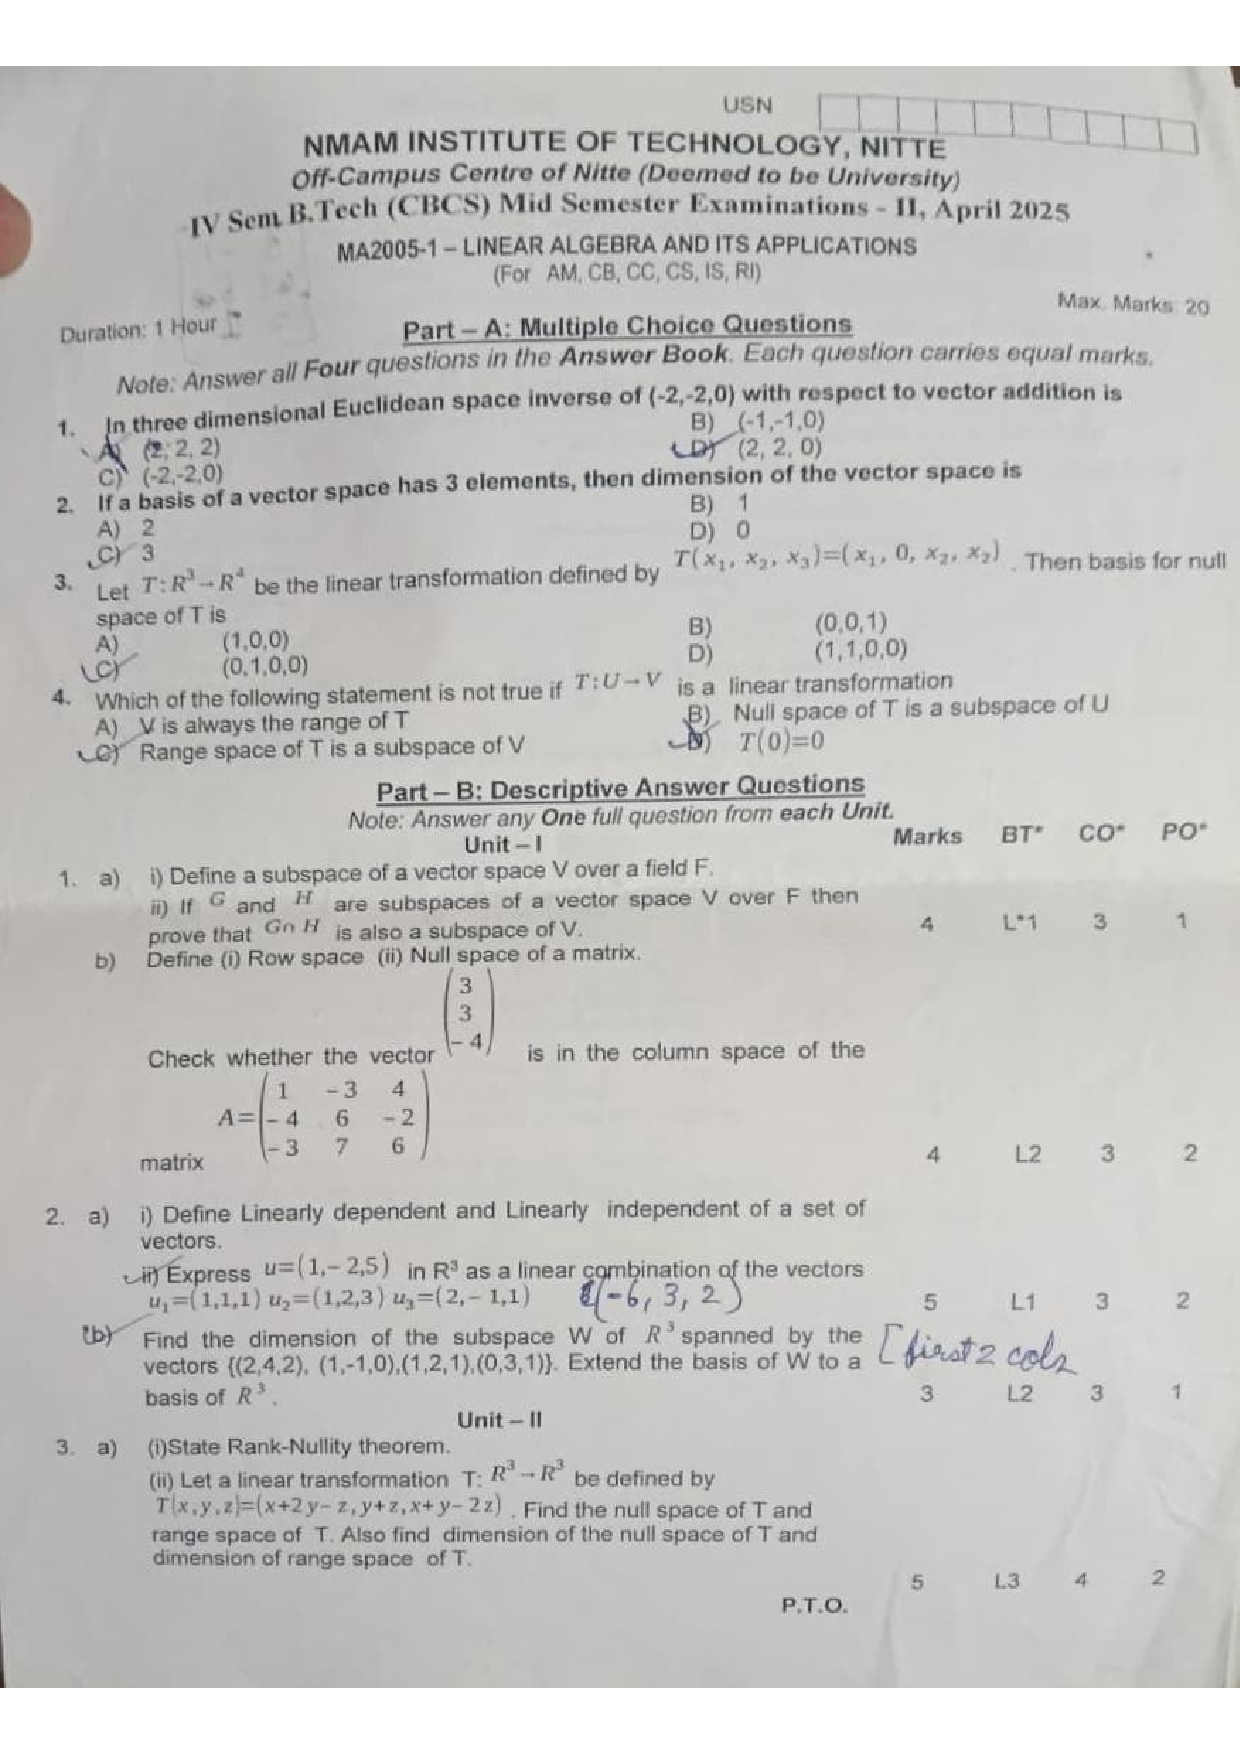
\includepdf[pages=-]{mse2_source.pdf}

% ========== PART 3: SOURCE EXAM BANK ==========
\bookmark[dest=part3,level=0]{PART 3: Source Exam Bank (33 pages)}
\hypertarget{part3}{}
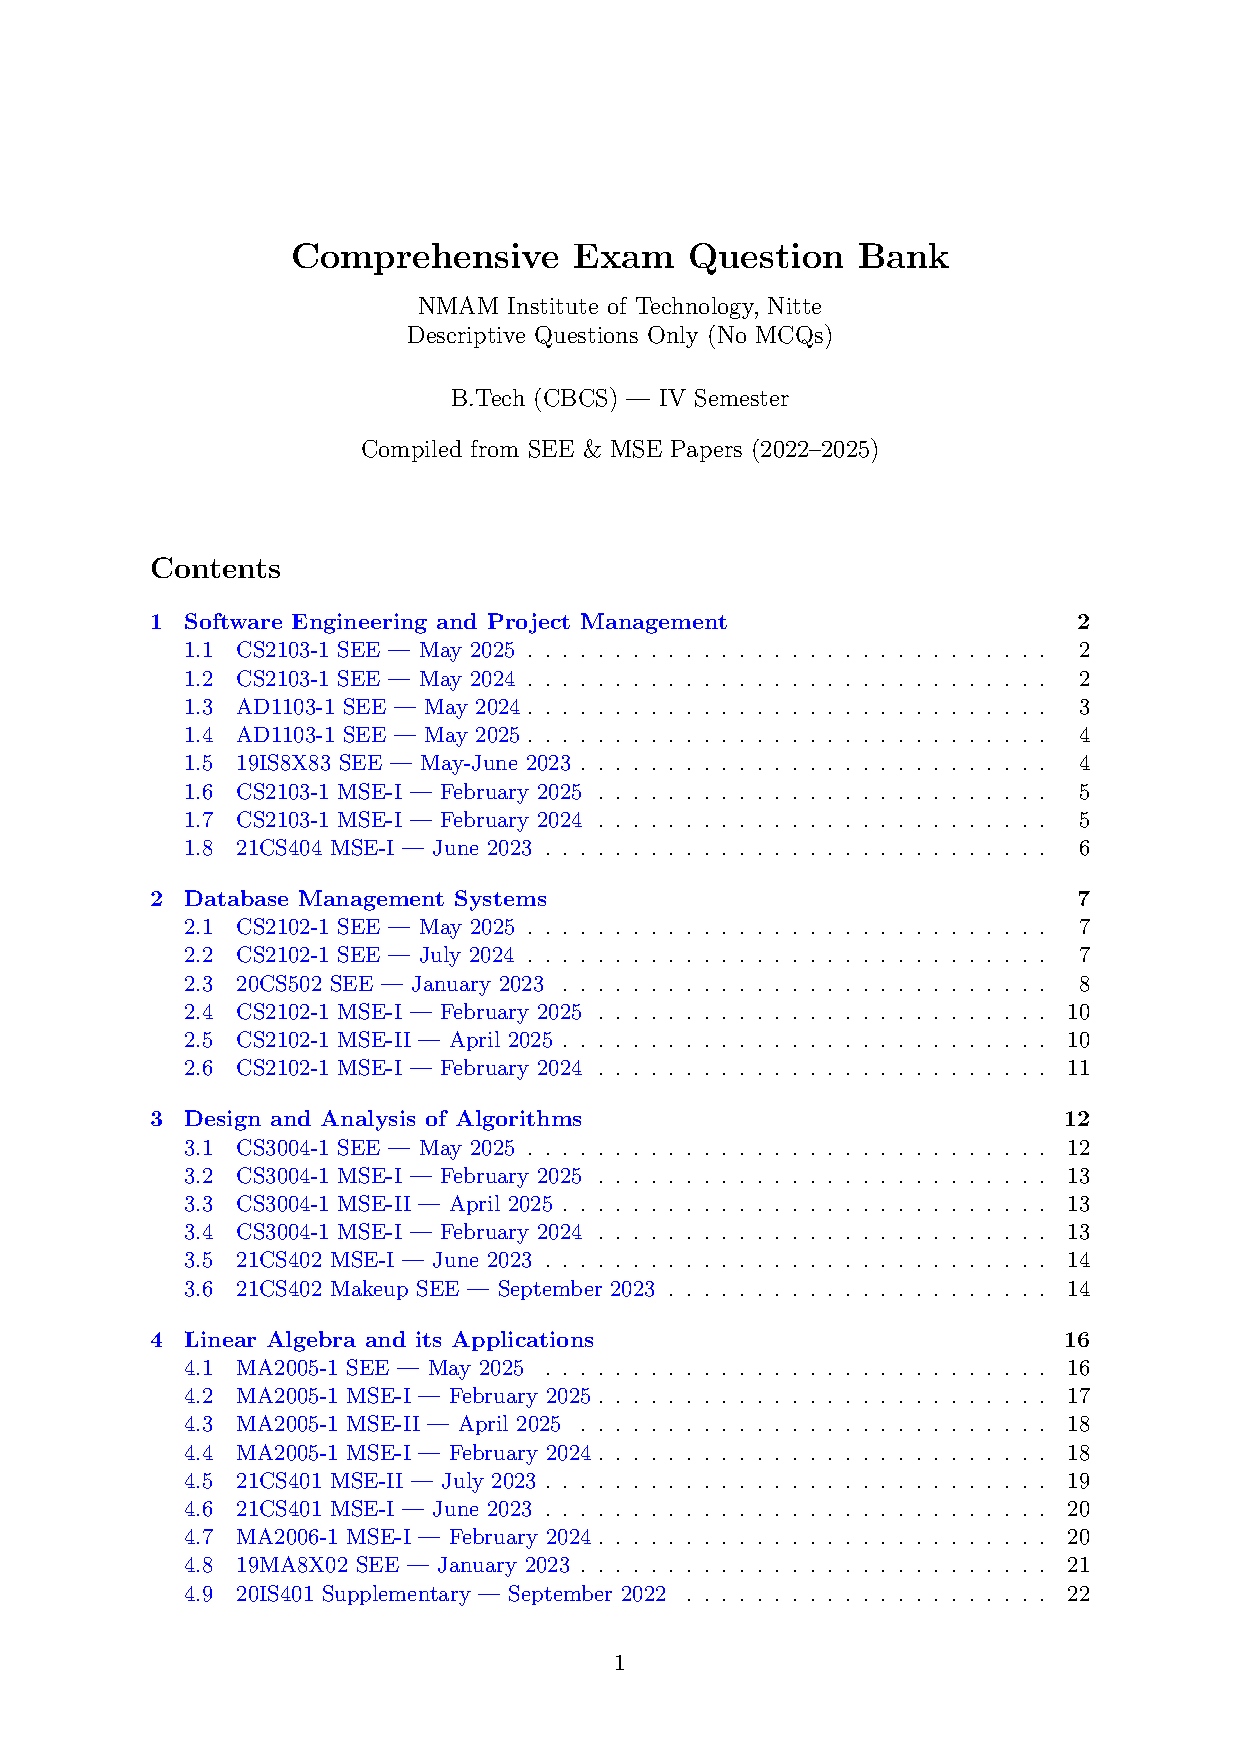
\includepdf[pages=-]{source_exam_bank.pdf}

% ========== PART 4: EXAM QUESTION BANK ==========
\bookmark[dest=part4,level=0]{PART 4: Exam Question Bank with MCQs (16 pages)}
\hypertarget{part4}{}

\includepdf[pages=-]{exam_question_bank.pdf}

% ========== PART 5: INDIVIDUAL PAPERS ==========
\bookmark[dest=part5,level=0]{PART 5: Individual Subject Papers (9 pages)}
\hypertarget{part5}{}

\bookmark[dest=part5.1,level=1]{Linear Algebra July 2023 (2 pages)}
\hypertarget{part5.1}{}
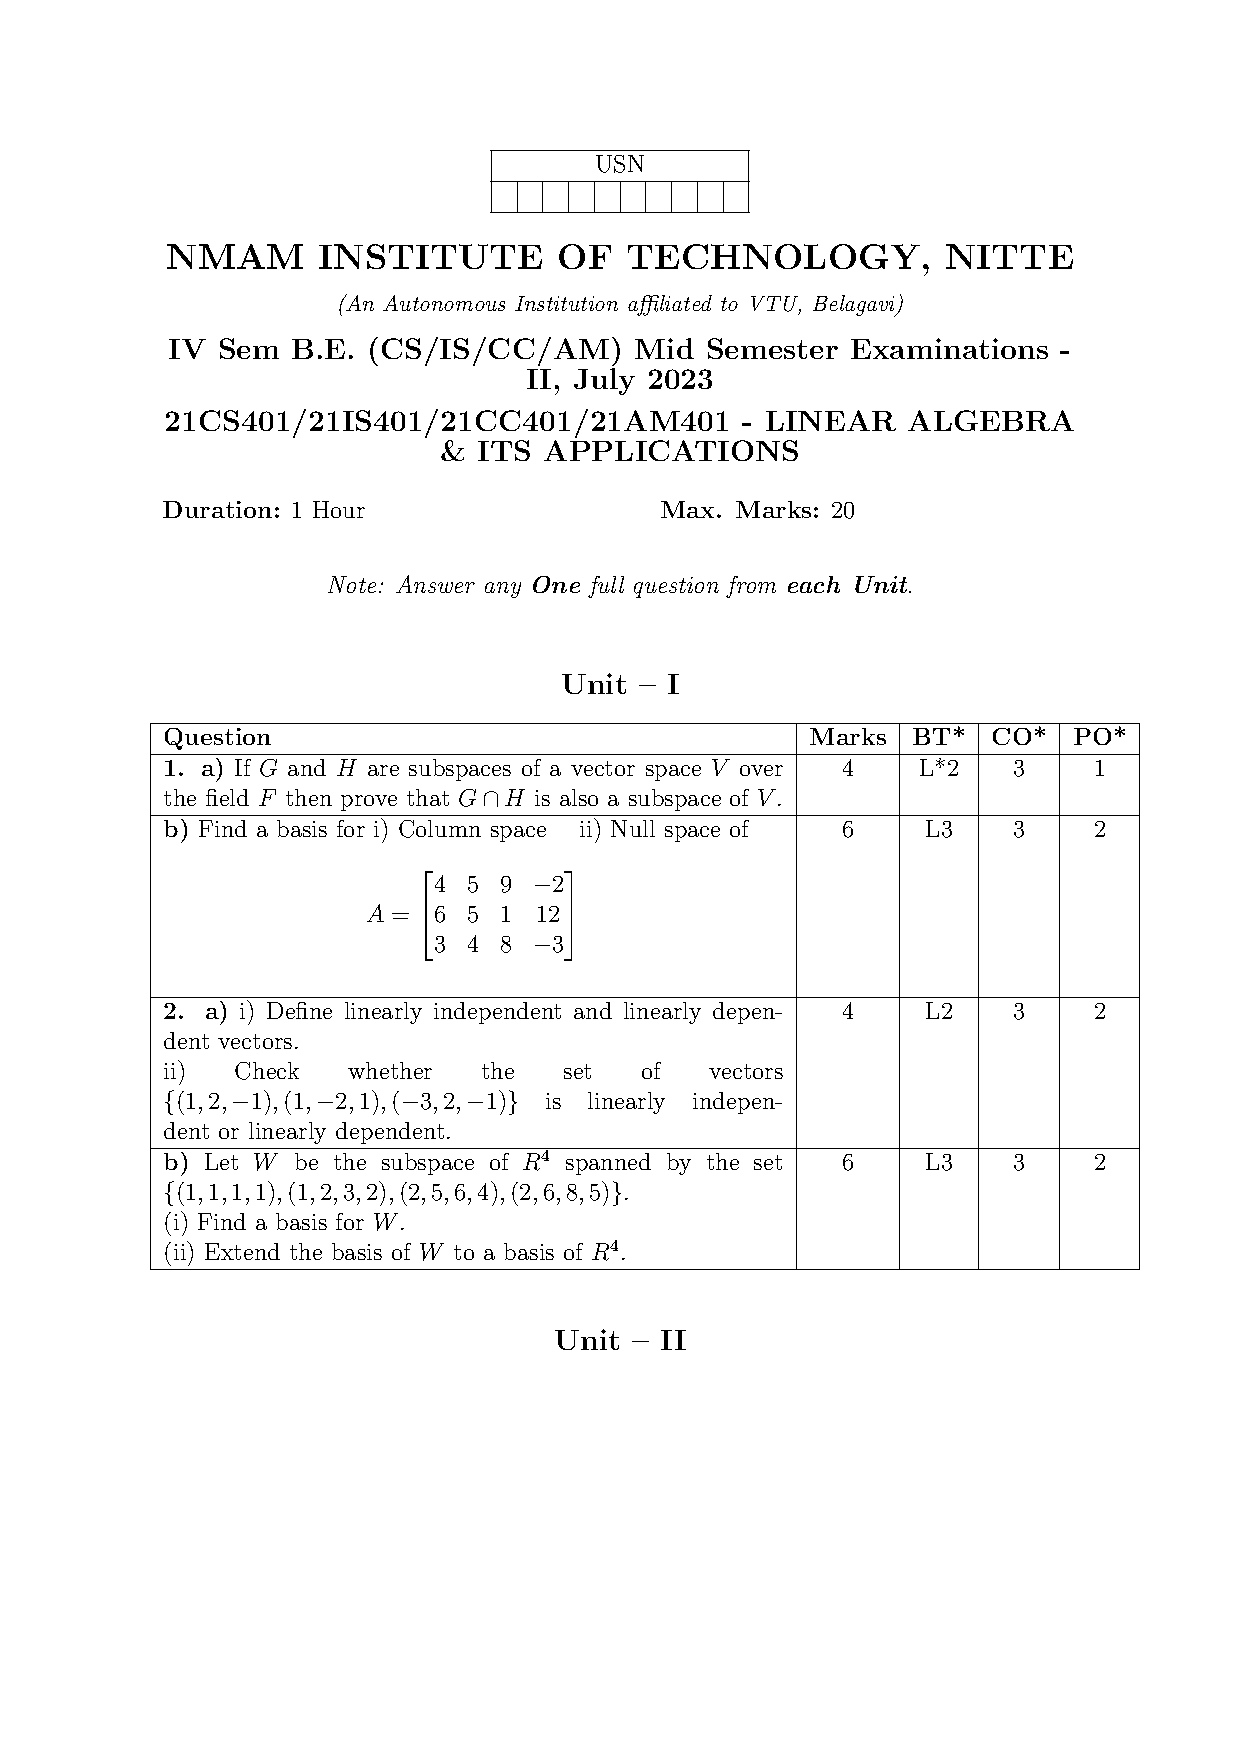
\includepdf[pages=-]{paper1_linear_algebra_july2023.pdf}

\bookmark[dest=part5.2,level=1]{DAA July 2023 (2 pages)}
\hypertarget{part5.2}{}
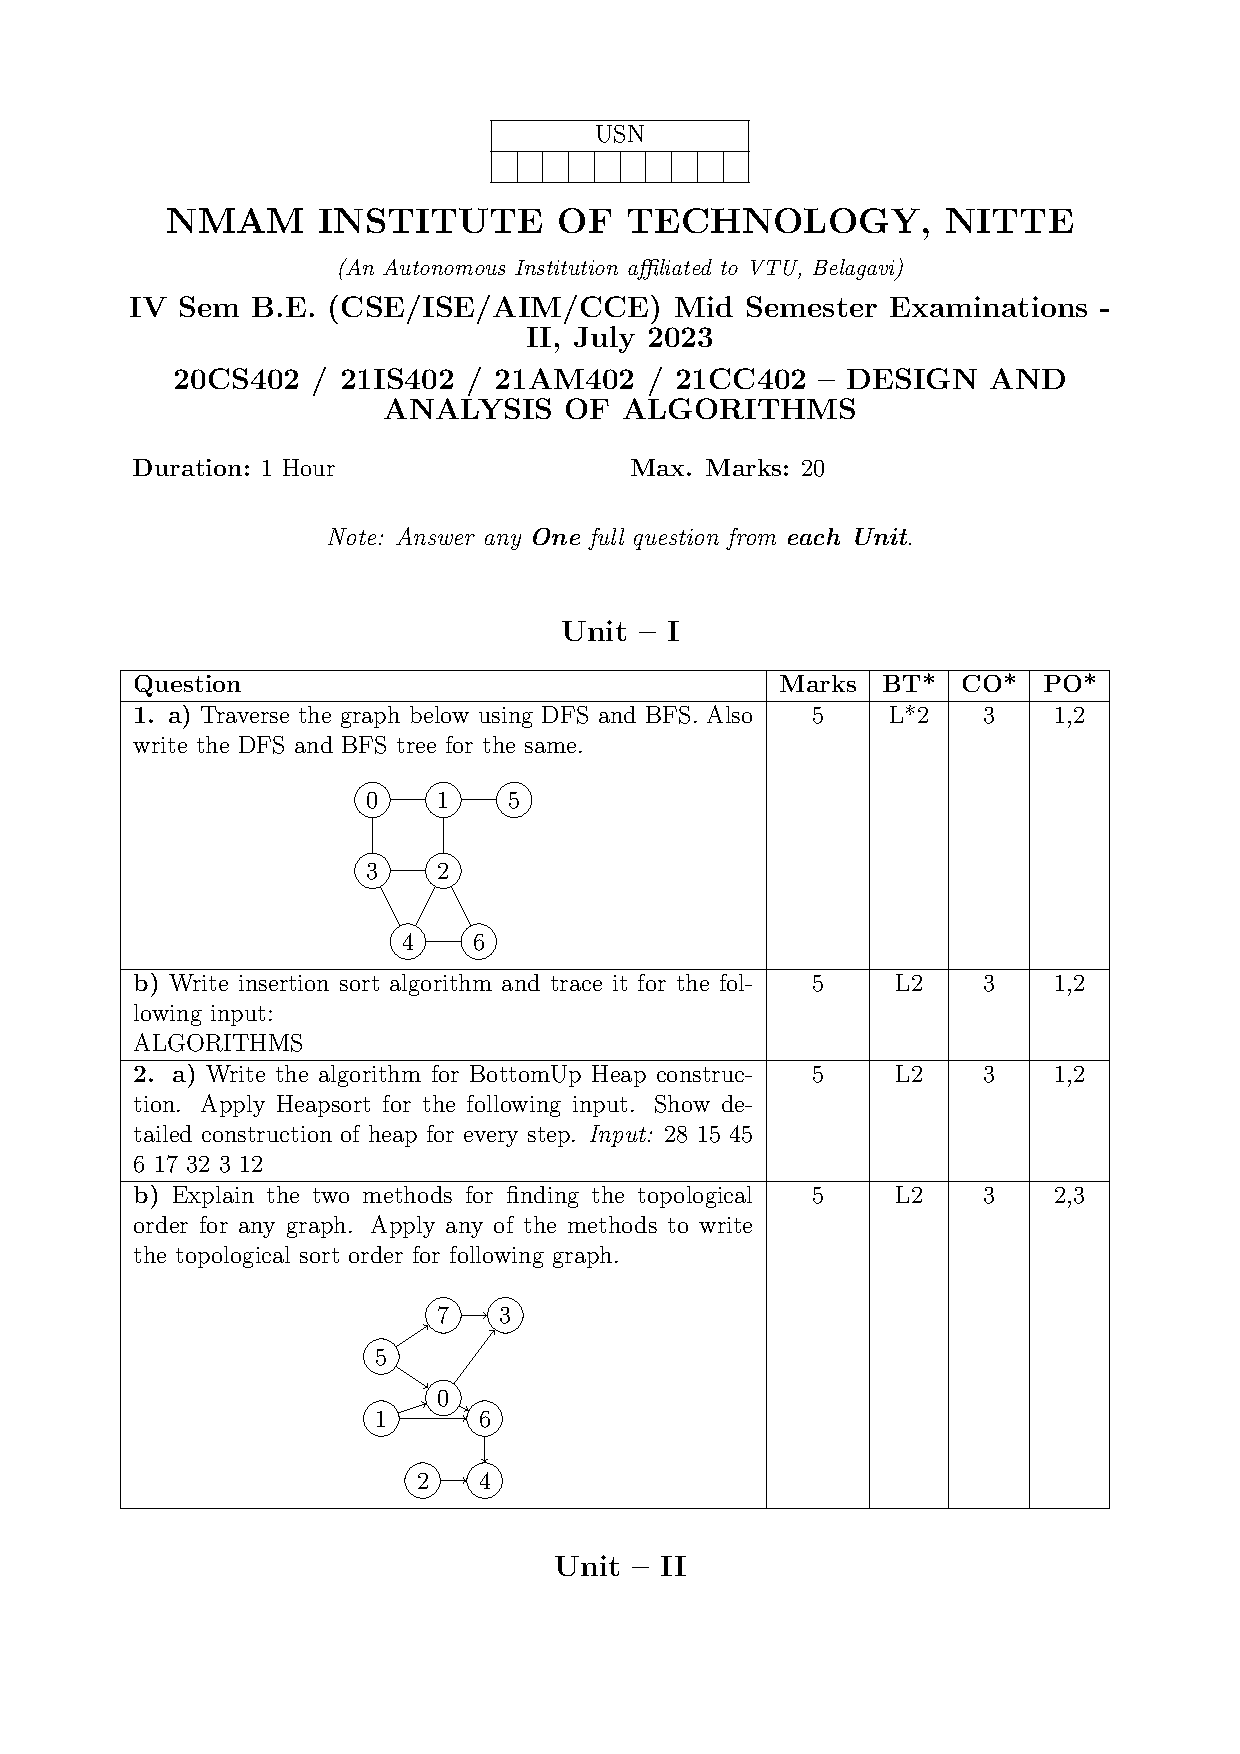
\includepdf[pages=-]{paper2_daa_july2023.pdf}

\bookmark[dest=part5.3,level=1]{Microprocessor July 2023 (1 page)}
\hypertarget{part5.3}{}
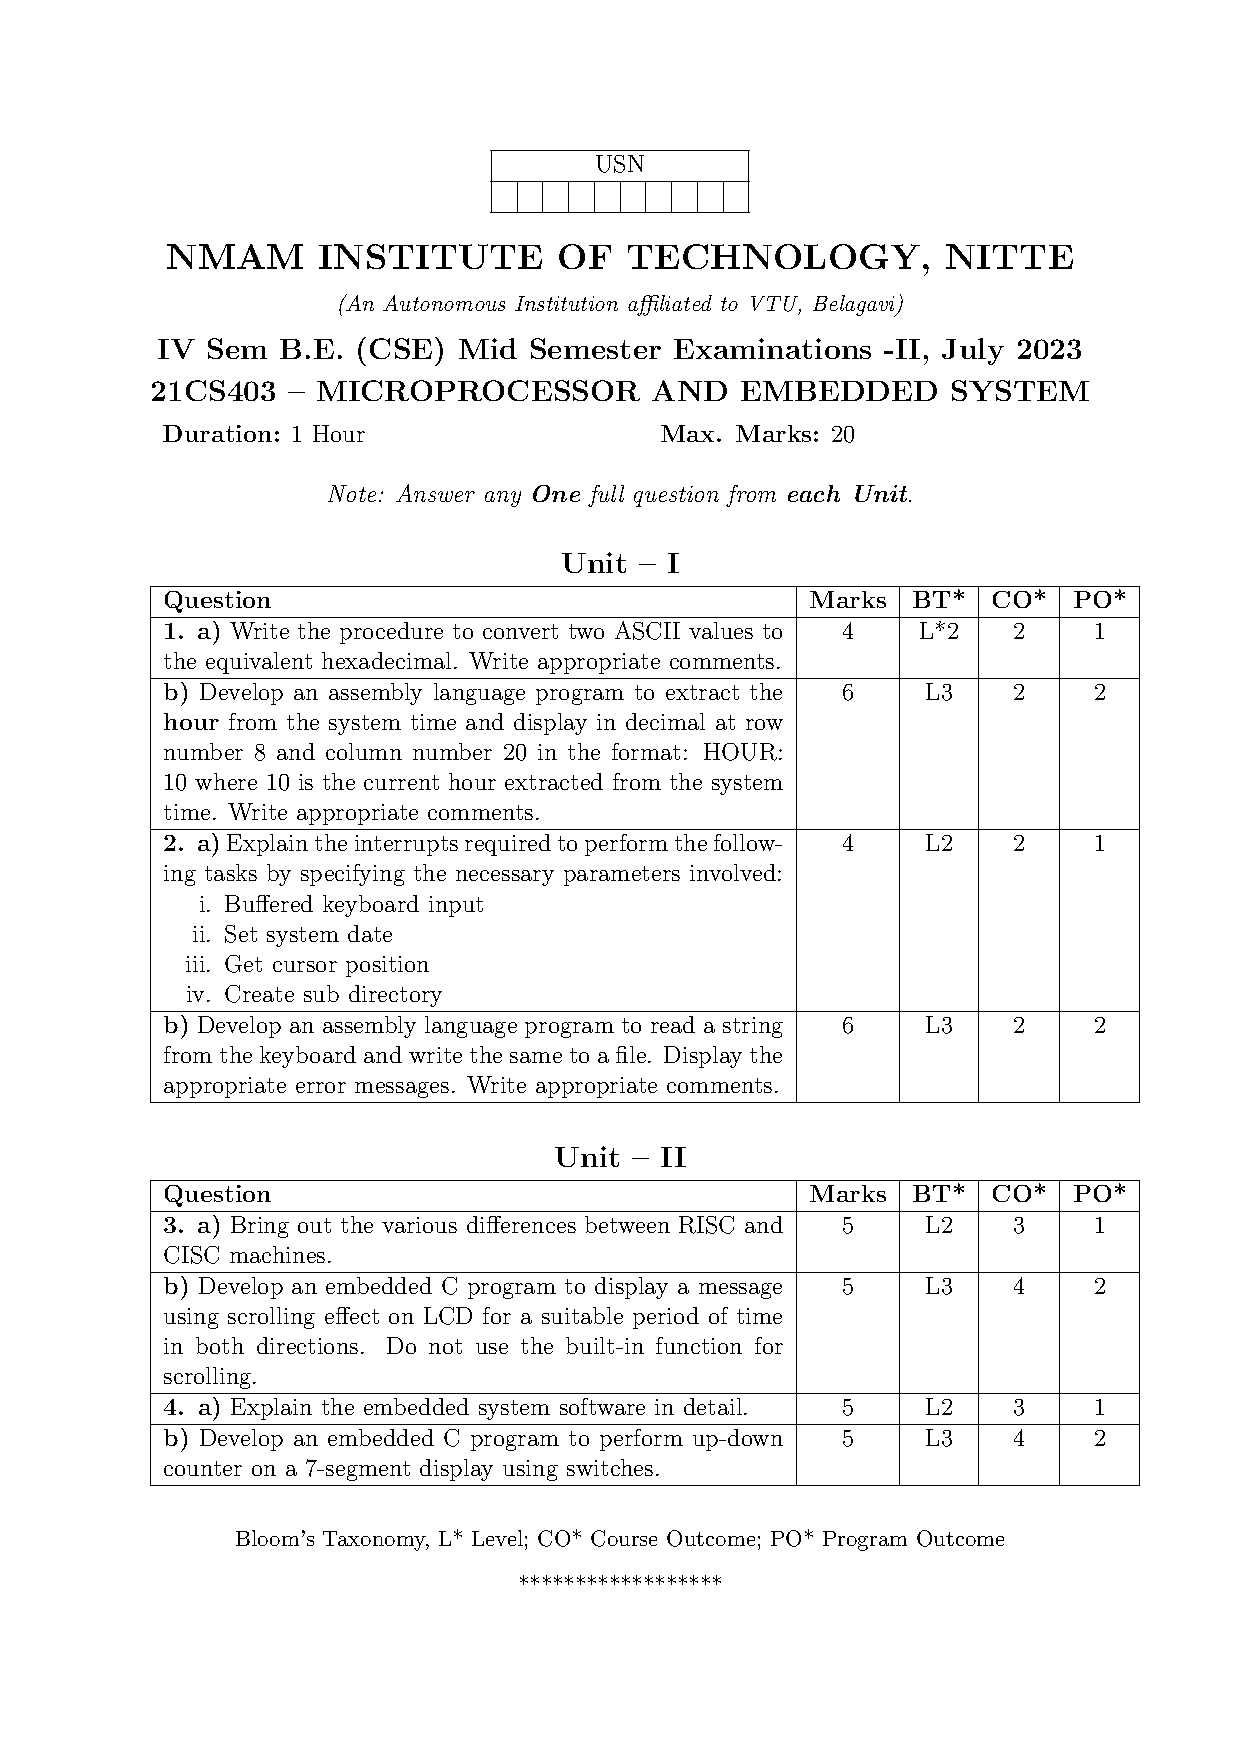
\includepdf[pages=-]{paper3_microprocessor_july2023.pdf}

\bookmark[dest=part5.4,level=1]{SEPM July 2023 (1 page)}
\hypertarget{part5.4}{}
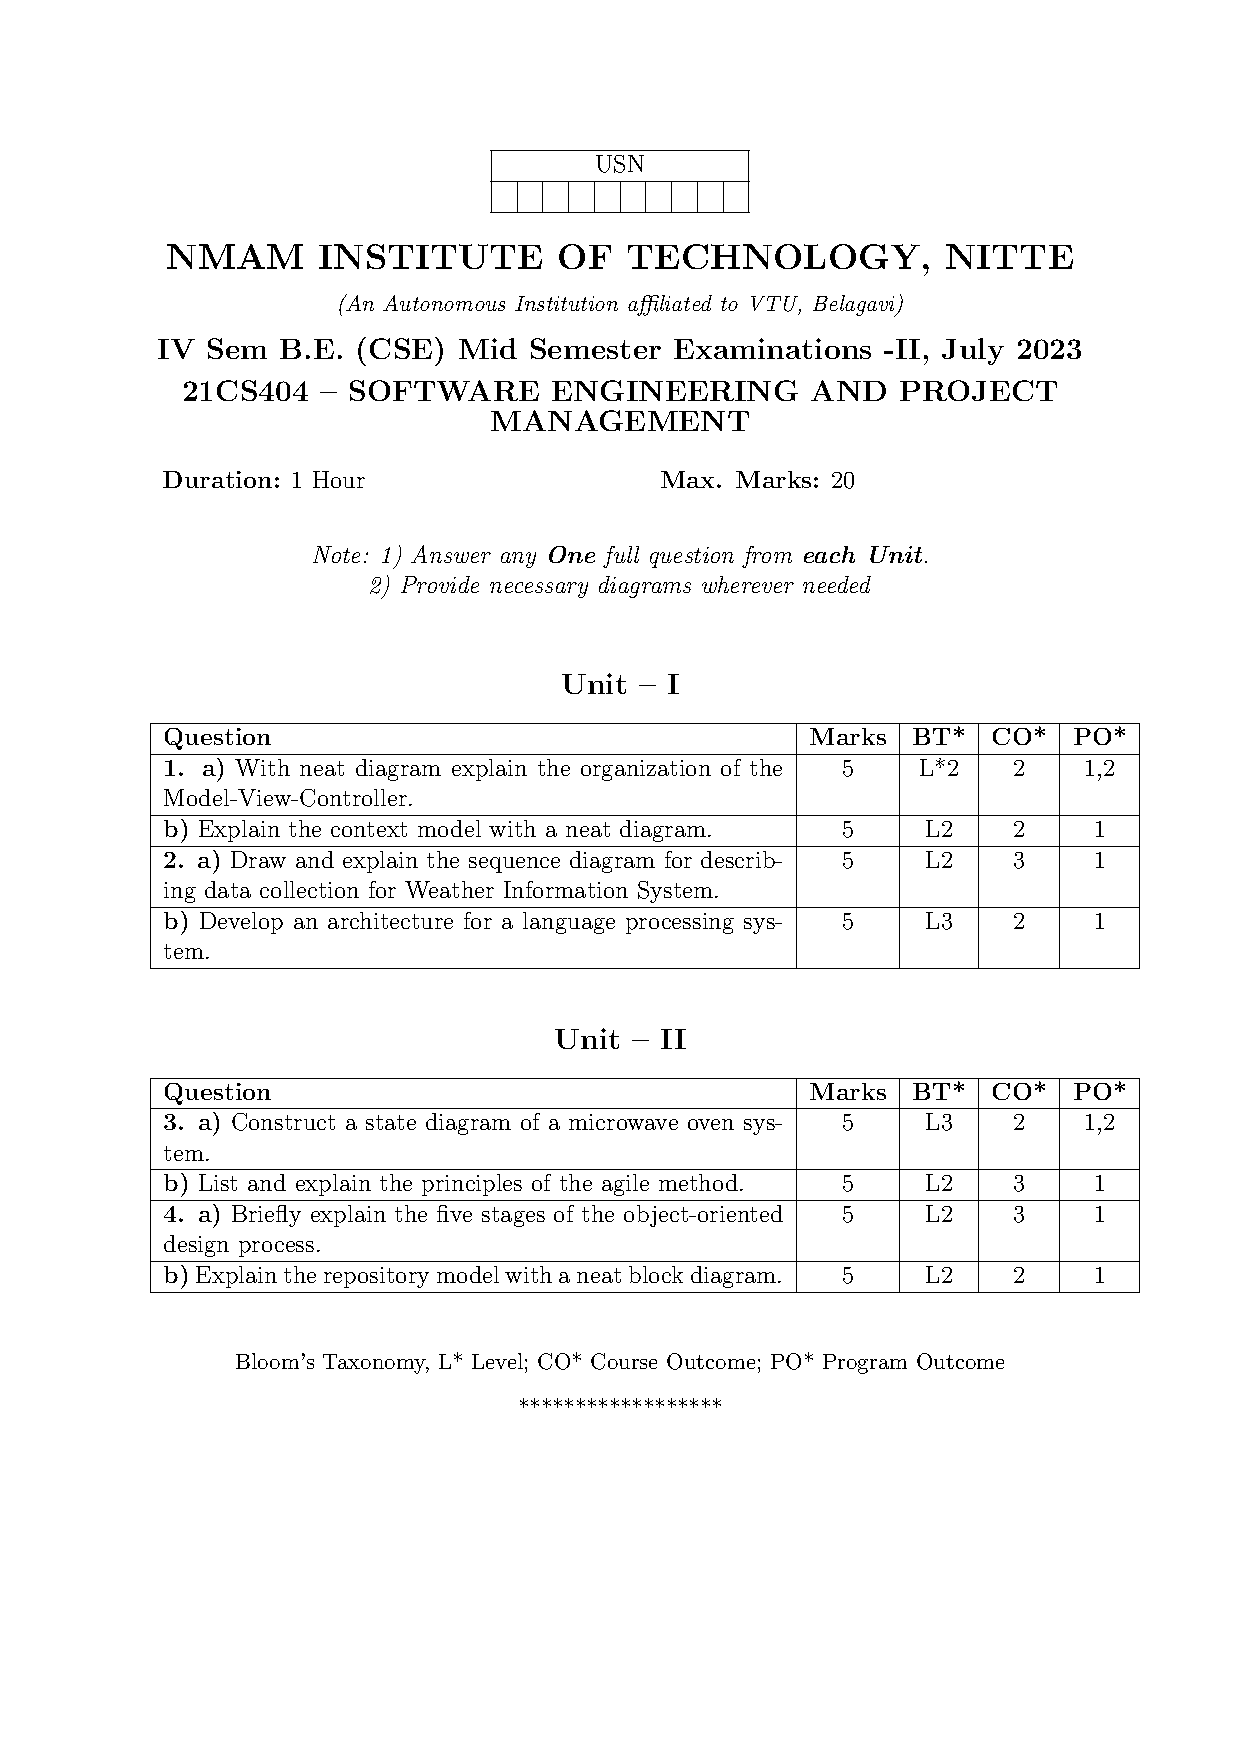
\includepdf[pages=-]{paper4_sepm_july2023.pdf}

\bookmark[dest=part5.5,level=1]{Linear Algebra June 2022 (2 pages)}
\hypertarget{part5.5}{}
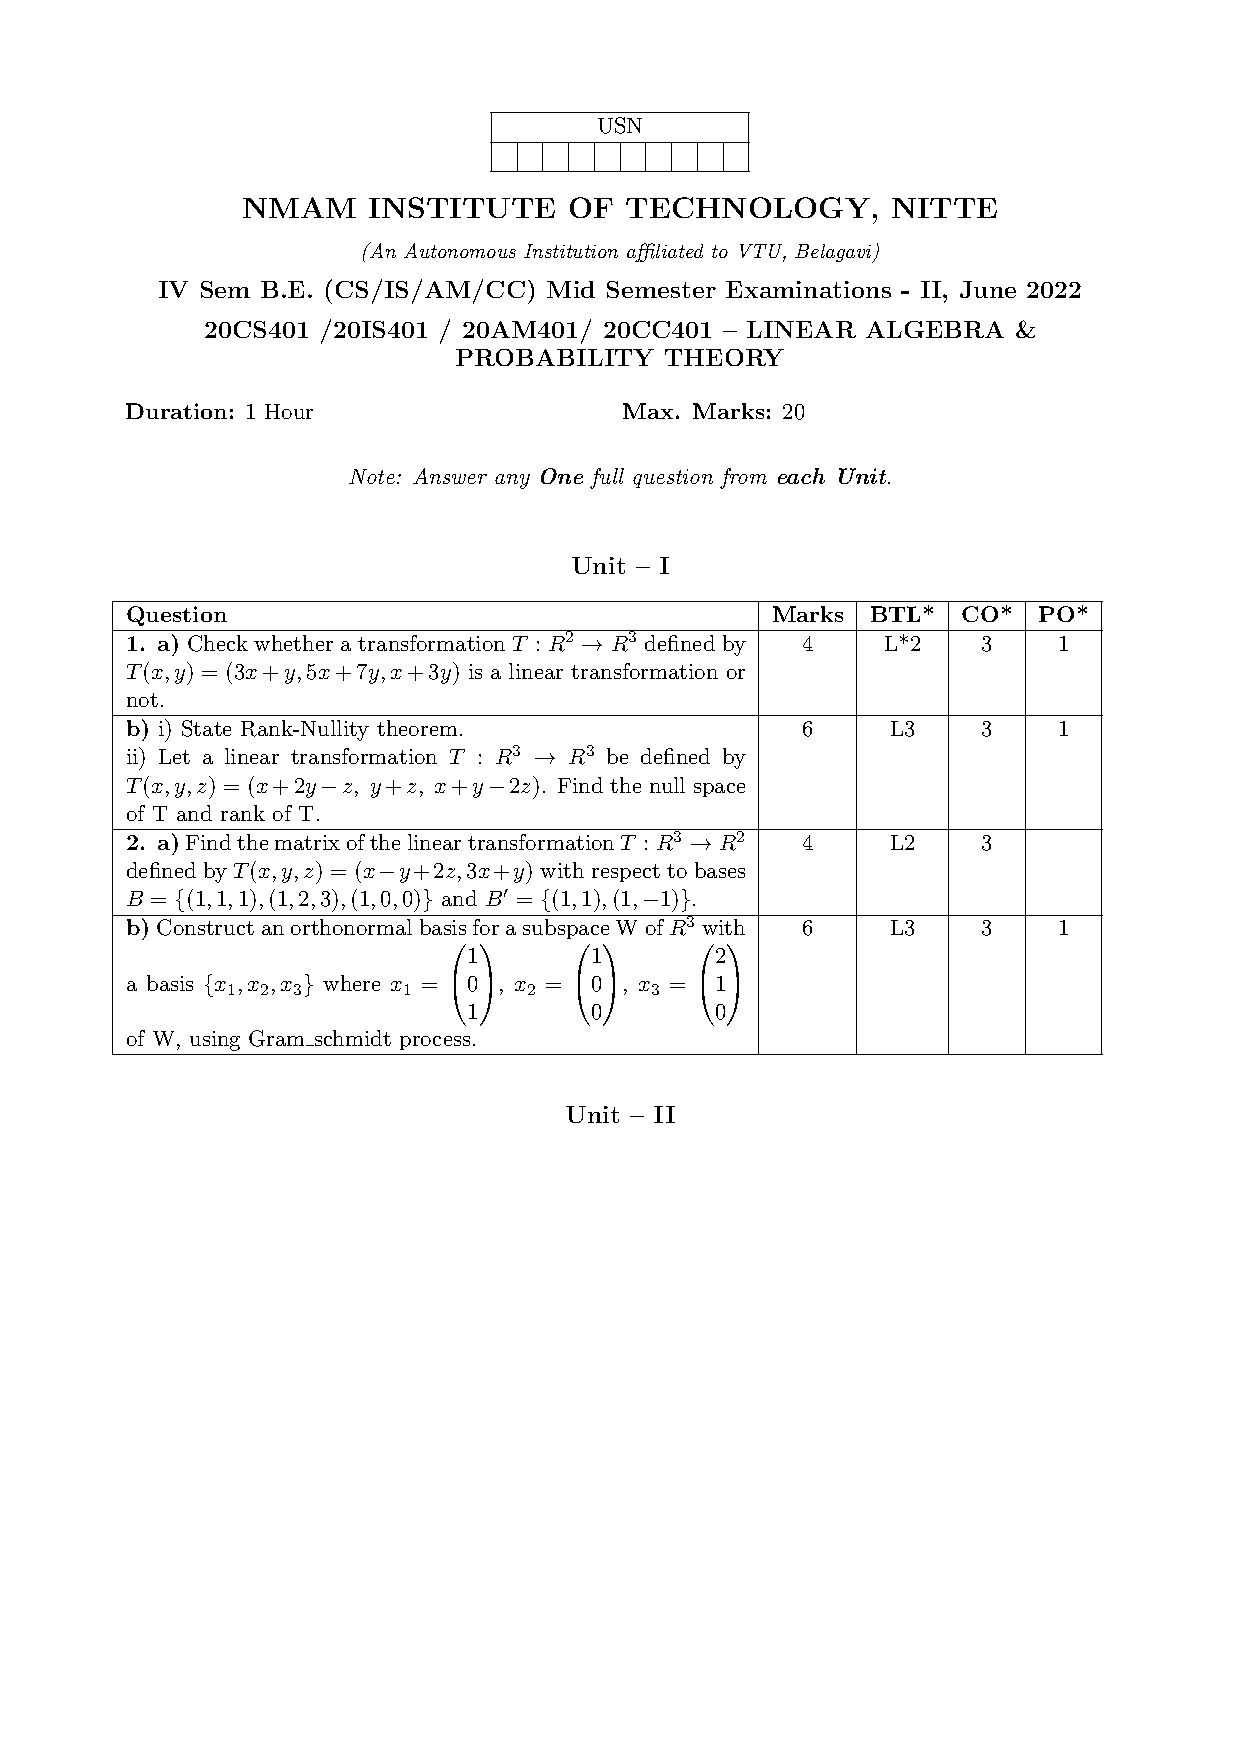
\includepdf[pages=-]{paper5_linear_algebra_prob_june2022.pdf}

\bookmark[dest=part5.6,level=1]{DAA June 2022 (1 page)}
\hypertarget{part5.6}{}
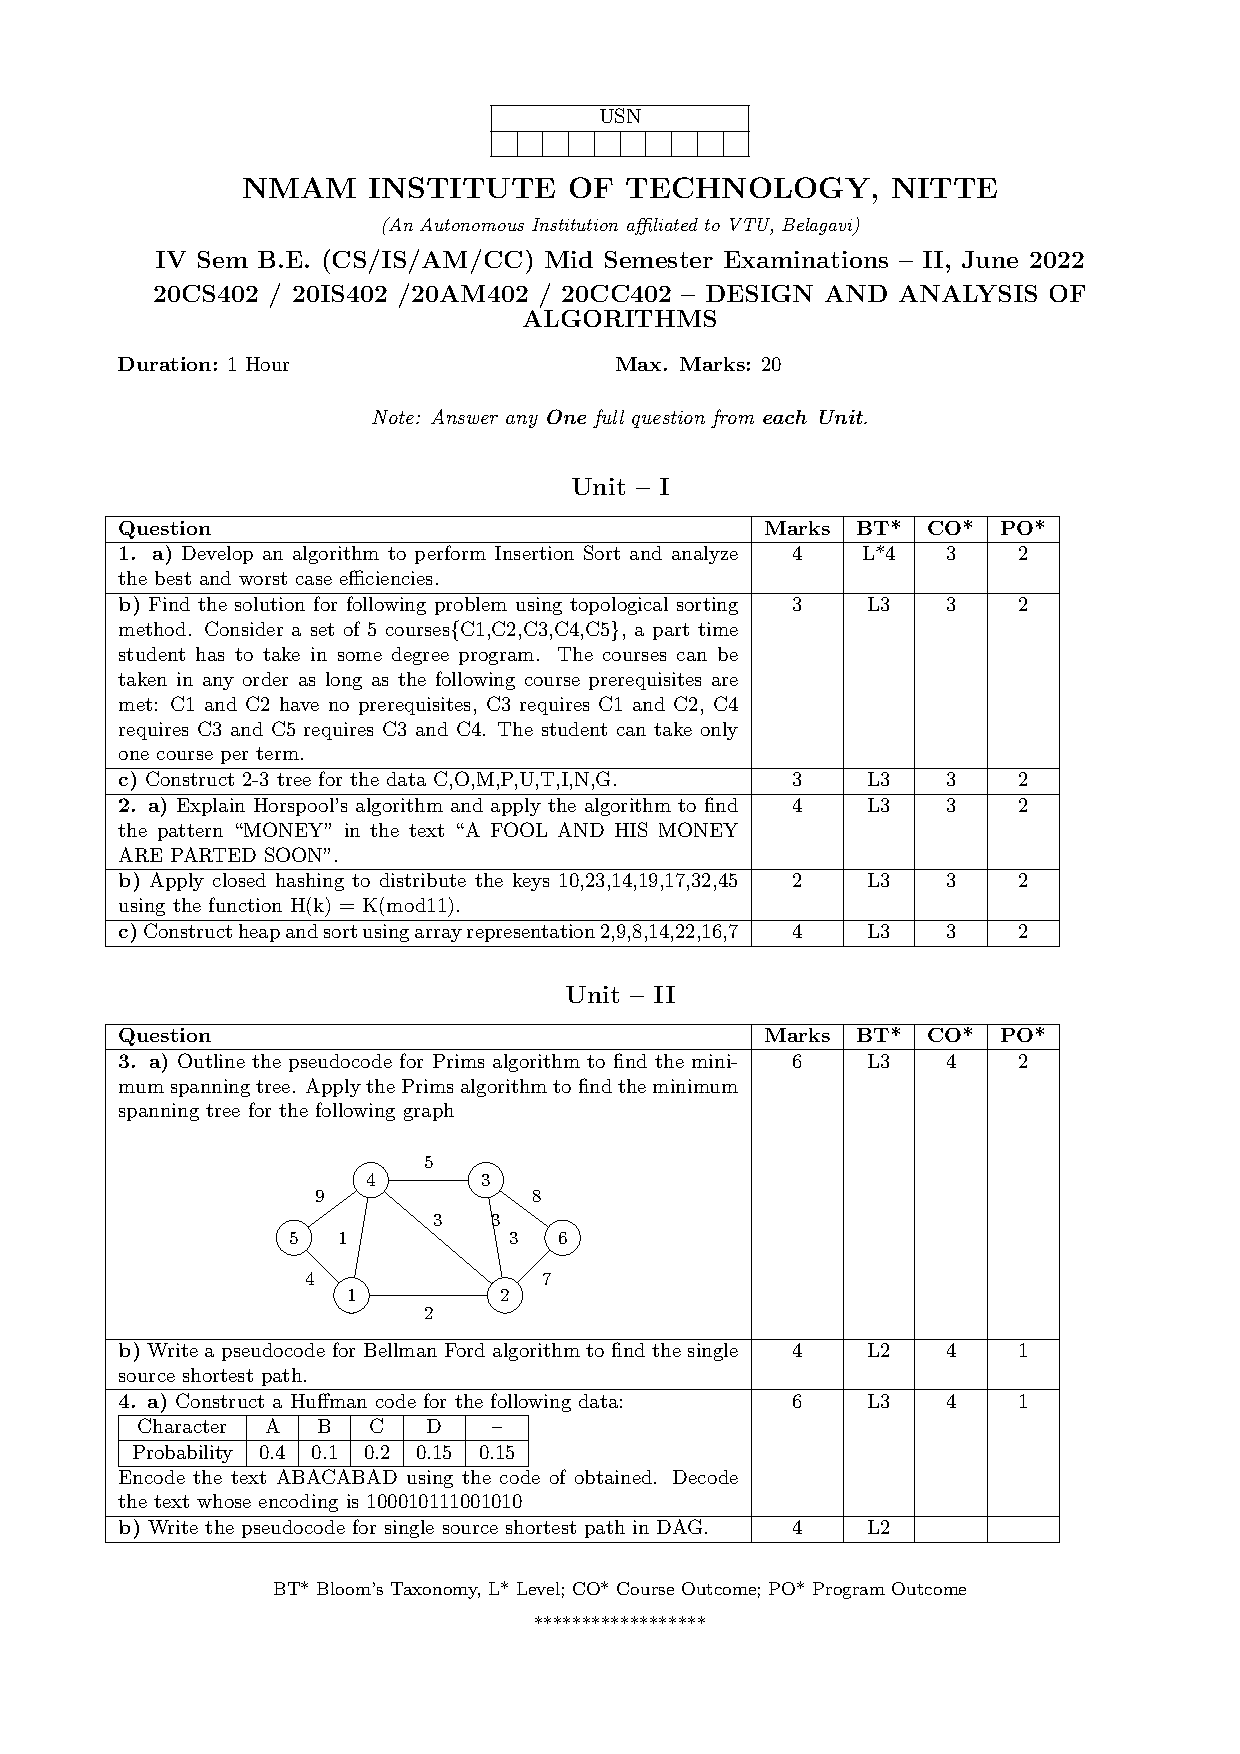
\includepdf[pages=-]{paper6_daa_june2022.pdf}

\end{document}
